\chapter{Results}

%\section{User Manual}

%\section{Technical Design}
In this section the technical design and implementation of the theory is described.
\section{Architecture and Design}
\label{sec:resultsarchitecture}
The final design of the architecture follows the basics of what was laid out in the initial design with some changes. These changes mostly concern the Application module which was initially planned to follow the Model-View-Controller architecture. The main reason for this is that the chosen GUI library acts as both view and controller. The Application module of the emulator will not be further explored in this section, instead the Game Boy module will be looked at in more detail.
\\\\
The Game Boy module is interacted with through the ``GameBoy''-class which also has the task of synchronising every part of the Game Boy emulation (see below). As mentioned in Chapter \ref{chap:Theory}, the different units communicate by reading from and writing to shared address space. This is reflected in the implementation as well as the diagram in Figure \ref{fig:dependency_diagram}, which is a dependency diagram of the Game Boy module.
\begin{figure}[H]
    \centering
    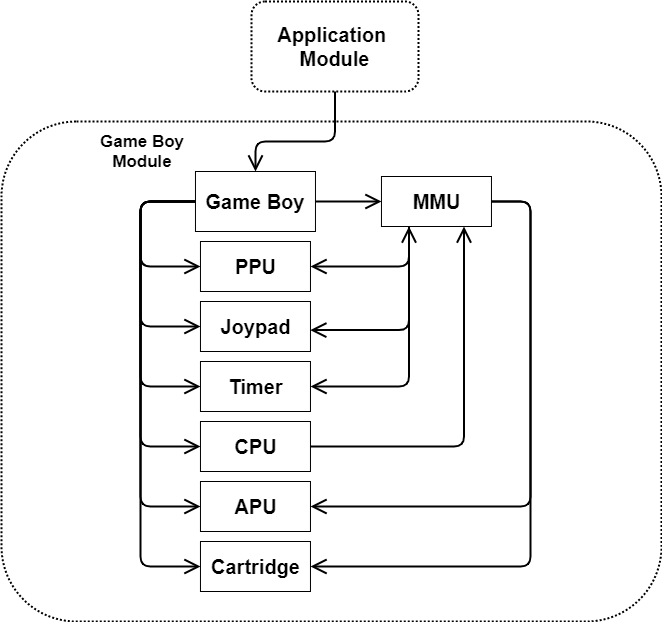
\includegraphics[scale=0.40]{figures/Game Boy Dependencies2.png}
    \caption{Dependency diagram over the Game Boy module.}
    \label{fig:dependency_diagram}
\end{figure}

Something which the original design knowingly did not take into consideration was the fact that the different hardware units run in parallel with different clock speeds. This choice was delayed as the research made showed that there were multiple possible solutions to synchronise the different units. Deciding which solution to implement therefore had to be done during development. The chosen solution was to make the CPU return the number of machine cycles after executing an instruction and to then allow the other units to catch up before executing another instruction, see Listing \ref{step}. The shown code snippet displays part of what could be considered the main loop of the emulation.
\\\\
\begin{lstlisting}[language=C++,
caption = {Code displaying how the CPU executes an instruction and returns the number of machine cycles, whereafter the other units catch up by executing the same number of cycles.},
label = {step}]
void GameBoy::step(IVolumeController *vc){
    ...
    int cycles = cpu->update();
    ppu->update(cycles);
    apu->update(cycles, vc);
    timer->update(cycles);
    cartridge->update(cycles);
    ....
    }
\end{lstlisting}
\newpage
\section{The Central Processing Unit}
\label{sec:CPUResults}
The implementation of the CPU mainly consists of translating the CPU instructions from assembly to a modern programming language, in this case, C++. The total number of instructions the CPU supports is 500 as mentioned previously, of which many are very similar to each other and all of which are implemented. Due to this, most of the instructions could be generalised into base functions, such as \texttt{add\_8bit} seen in code in Listing \ref{addA}. These base operations could in turn handle the variation of the instructions and instead of implementing one function for each operation code, the correct input simply needed to be provided to the correct base instruction given an operation code. There are some exceptions, amongst them the HALT-instruction \cite{HALT-behaviour} which has a very particular behaviour and therefore needed to have a separate implementation.
\\\\
\begin{lstlisting}[language=C++,
caption = {Code displaying a generalised method used, in this case an addition function which allows for addition between register A and all other registers, both with and without the use of the carry bit.},
label = {addA}]
void CPU::addA(uint8_t value, bool withCarry) {
    add_8bit(A, value, withCarry);
}

void CPU::add_8bit(uint8_t &a, uint8_t b, bool withCarry) {
    auto CFlag = withCarry ? F.c : 0;
    setCFlag(a, b + CFlag, false);
    setHFlag(a, b, false, CFlag);
    a += b + CFlag;
    //Note that all 'false' parameters specify that subtraction is not used, which in turn affects how and which flags are set.
    setZNFlags(a, false);
}
\end{lstlisting}

\subsection{Interrupts}
As previously stated, the CPU has five types of interrupts. Of these five only the ``Serial interrupt'' is not implemented, which there never was any intention of implementing as mentioned in Section \ref{sec:Delimitations}. All the implemented interrupts are in some ways central in having a working CPU as these allow for other units to request the CPU to perform specific tasks when needed.
\newpage
\subsection{Testing of the Central Processing Unit}
Mainly, three tests were used for checking the accuracy of the CPU. These check the correctness of the instructions \cite{Blargg}, their timings and the interrupt timing respectively. The tests regarding the CPU-instructions, \texttt{cpu\_instrs} and \texttt{instr\_timing}, pass on both the real hardware \cite{TestROMsResult} and the emulator see Figure \ref{fig:cputests}. The \\\texttt{interrupt\_time} test, however, does not pass despite being implemented and performing as expected. It most likely fails due to the implementation of the synchronisation of the different units. This is further discussed in Section \ref{sec:CPUDiscussion}. 

\begin{figure}[H]
\centering
\begin{subfigure}{.5\textwidth}
  \centering
  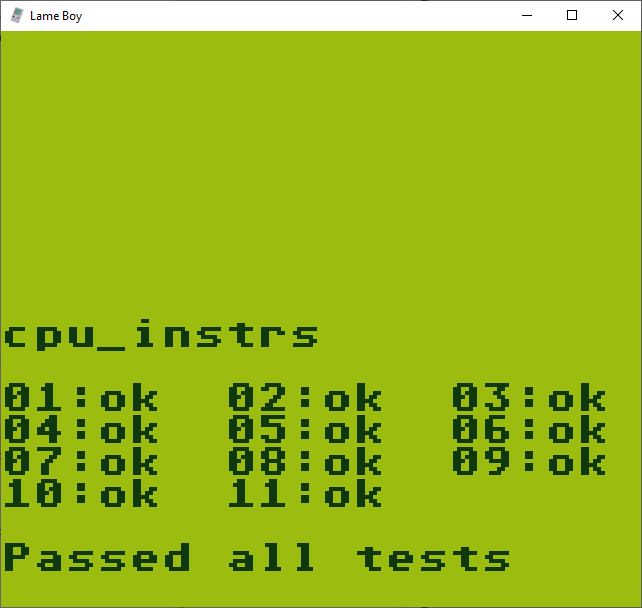
\includegraphics[width=0.9\linewidth]{figures/cpu_instrs_passed.PNG}
  %\caption{Figure displaying the emulator passing Blargg's test checking the correctness of the CPU instructions.}
  %\label{fig:cpu_instrs}
\end{subfigure}%
\begin{subfigure}{.5\textwidth}
  \centering
  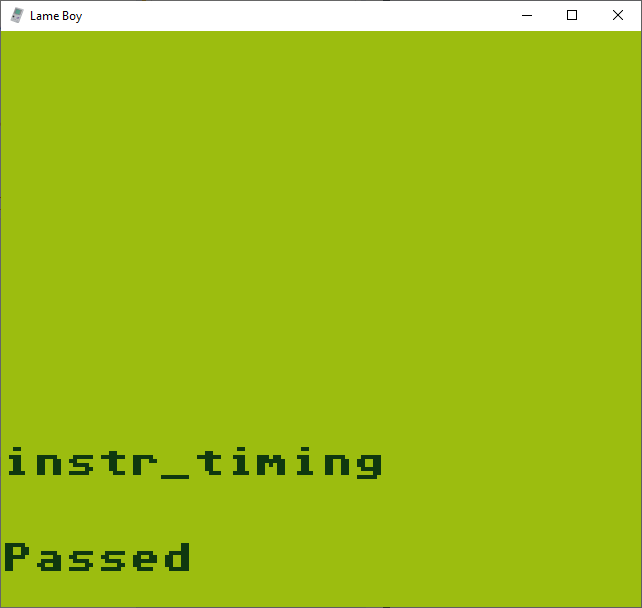
\includegraphics[width=0.9\linewidth]{figures/instr_timing_passed.PNG}
 % \caption{Figure displaying the emulator passing Blargg's test checking the correctness of the CPU timing.}
  %\label{fig:instr_timing}
\end{subfigure}
\caption{Displaying the emulator results from  Blargg's test ROMs checking the correctness of the CPU instructions and CPU timing respectively.}
\label{fig:cputests}
\end{figure}   

%There are a number of additional test ROMs, amongst them mooneye-gb \cite{Gekkio-Mooneye}. Many of these have not been run on the emulator as of yet, and no results from these can therefore be presented. However, as the CPU is passing the most central tests, the ones regarding instruction correctness and timing; which affect not only the CPU but all hardware units, further work regarding improvement of the accuracy of the CPU was put on hold.
\newpage
\section{The Memory Managing Unit}
The Game Boy uses memory mapped I/O which means that almost all communication can be done through reading and writing to the different addresses. Therefore the main purpose of the MMU is to provide functionality which supports reading memory and writing to memory. 
%Because the Game Boy uses memory mapped I/O almost all communication can be done through reading and writing to the different addresses.
%Therefore the main purpose of the MMU is to have a read and a write function which in turn calls a specific device's read and write function.
%The read function is supposed to return the value on the given address. The write function is supposed to write the given value to the given address.
\\\\
To separate code and improve the possibility for parallel development all the different devices are separated into their own classes: PPU, APU, Cartridge, Joypad and Timer, each having their own read and write functions. 
The memory addresses used by the device (mostly control registers) are also maintained in the devices' class. 
The other memory areas which are not part of a device are located directly in the MMU class. Examples of such memory are: boot ROM, VRAM, WRAM, OAM, and HRAM.

\subsection{Timer}

The timer is implemented as a device with read and write functions. 
Reading and writing to the timer's four registers is implemented to behave as described in the Section \ref{sec:MMUTheory}.  
To make the timer update at the same pace as the CPU (and the system as a whole) it has an update function. 
The update function allows the timer to catch up to the system based on the number of cycles required for the last CPU instruction executed, see Section \ref{sec:resultsarchitecture}.
Because of the timer not being updated continuously it is not always accurate. On original hardware the counter would increase during the execution of a CPU instruction and could therefore change between the start of the execution and the actual read from the counter register.


% Updated based on the cpu instruction.
% Not completely accurate, (skipping counts).


\subsection{Cartridges and Memory Bank Controllers}
Due to the fact that there are a number of different game cartridges, all supporting different hardware, such as different MBCs, RTC, ROM and XRAM sizes, a modular approach was taken. 
This was possible as although the cartridges may have different hardware they operate in a similar manner, therefore an MBC interface class was made.
This enables different behaviour when reading or writing to the cartridge's addresses depending on the used MBC. The MBC interface also uses an update function to allow the possibility of an RTC to update at the same pace as the rest of the system. This function updates the RTC according to the specified number of clock cycles, see Section \ref{sec:resultsarchitecture}. For MBCs without an RTC this function does not do anything. This way multiple MBC classes can be implemented to easily expand the support for different MBCs. The most common MBCs are MBC1 and MBC3, which are also the ones which have been implemented.
%The MBCs that are used in most common games are the MBC1 and MBC3 which is the ones that have been implemented.
\newpage
The information about hardware used in each game is stored in the game ROM file.
When loading the ROM file into memory the MBC type, ROM size and XRAM size can be obtained and initialised accordingly. 
Another feature for games with XRAM supported with a battery is the ability to save data between different sessions.
A common way to support this in emulators, this one included, is to create a separate file to save the current contents of the XRAM to. Meaning that when loading a ROM file, the emulator also looks for an XRAM-file, which if found is also loaded and initialised, providing a way to use a games' built in save functionality.

\subsection{Testing of the Memory Management Unit}
Testing of the implemented MBCs has been done using test ROMs that test different features of the MBC such as ROM and XRAM bank switching as well as the RTC. The MBC tests used are Gekkio's mooneye-gb tests \cite{Gekkio-Mooneye} and aaaaaa123456789's rtc3test \cite{mbc3test}, which the emulator pass.
\\\\
Testing the timer was done with some test ROMs from Gekkio's mooneye-gb tests \cite{Gekkio-Mooneye}. Most of them did not pass, most likely due to the inaccuracies caused by the update function. Although, its basic counting capability has been tested through games that for example use the counter to produce randomness. Without the counter the supposed randomness did not produce different outcomes, but with the timer implemented the outcome seemed more random.

% Passing a couple of tests but fail most of them. Probable because inaccuracy in updates. Works for randomisation in Tetris.
\newpage
\section{The Pixel Processing Unit}
The PPU class aims to replicate the functionality of the PPU in the Game Boy. In this section, the term ``PPU'' will refer to the PPU class and the term ``original PPU'' will refer to the Game Boy's PPU.\\
\\
The PPU contains the same registers as the original PPU and implements read and write methods that the CPU uses to communicate with the PPU.

\subsection{Timing}
As mentioned in Section \ref{sec:resultsarchitecture}, the PPU is controlled by a different clock than the CPU and need to be kept in sync. To solve this problem, the PPU is updated every time a CPU instruction is executed. By providing the number of cycles the CPU instruction used to the update-method of the PPU, it is possible to determine how much time has passed since it last switched mode and thereby decide whether the PPU should switch mode or not. For simplicity, the PPU also does all the real ``work'' of a mode whenever it switches from that mode.

\subsection{Basic operation}
The basic operation of the PPU is described by the update-method. Firstly, the PPU adds the number of cycles elapsed since the last CPU instruction was executed to the number of accumulated cycles since the PPU last switched modes, as seen in Section \ref{sec:resultsarchitecture}. It then checks whether or not it should switch mode. This calculation is based on the durations in Table \ref{tab:PPU_mode_durations}; That is, the draw mode has been set to take the fewest amount of cycles that it can possibly take in the real Game Boy and the H-blank has been set to take as much time as is possible. When this is done, the PPU checks whether a STAT-interrupt should be requested and if so requests one.
\begin{table}[H]
    \centering
\begin{tabular}{l|l}
    \textbf{Mode} & \textbf{Cycles} \\
    \hline
    H-blank & 51\\
    V-blank & 144\\
    OAM-search & 20\\
    Drawing & 43
\end{tabular}
\\\
    \caption{The durations of the PPU's modes}
    \label{tab:PPU_mode_durations}
\end{table}
What happens when the PPU changes mode depends on which mode it was just in. This is very similar to the basic operation described in Section \ref{sec:PPU_Modes} but there are a few differences, the main ones being that the image is rendered one line at a time and that the CPU has free access to VRAM and OAM at all times. The operation during the various modes is described below.\\
\\
\newpage
\textbf{H-blank}\\
When leaving an H-blank, the PPU moves on to the next scanline. The LY register is therefore increased by one. If all lines have been drawn, the PPU moves to V-blank mode and a V-blank-interrupt is requested. If not, the PPU goes into OAM-search mode.\\
\\
\textbf{V-blank}\\
The V-blank in the emulator is treated as ten blank scanlines, since the V-blank in the Game Boy lasts for ten lines. Therefore, the LY register is increased by one every time the PPU is done with a blank scanline. If all ten blank scanlines have passed, LY is reset to 0 and the PPU goes into OAM-search.\\
\\
\textbf{OAM-search}\\
When leaving OAM-search the PPU prepares the sprites to be drawn on the current line by adding the ones that intersect with the line to a priority queue. This ensures that when retrieving the sprites from the queue, the ones with highest priority will be drawn above those with lower priority. The PPU then goes into drawing mode.\\
\\
\textbf{Drawing}\\
When leaving the drawing mode, the PPU processes the next line by calling the \texttt{processNextLine} method and then goes into H-blank mode. The drawing process is described in detail in Section \ref{sec:result-drawing}.

\subsection{Drawing}
\label{sec:result-drawing}
Unlike the original PPU, which draws pixels directly to the LCD, the PPU instead inserts pixels into a frame buffer. Scanlines are drawn one at a time, but the layers background, window and sprites are drawn in that order on top of each other, depending on which of these layers are enabled in the LCDC register.\\
\\
\textbf{Background}\\
For a given scanline, for each x-coordinate, the PPU determines the tile corresponding to the coordinate, then which pixel of the tile should be drawn and lastly which colour it should have. The colour is written to the frame buffer and the colour index is saved in an array containing the background and window colour indexes for the current line. This array is later used for determining sprite priority over the background.\\
\\
\textbf{Window}\\
For a given scanline, the PPU first determines whether the window covers this scanline. If it does, the window pixels are written to the frame buffer in a similar manner to how the background is written. Any background pixels covered by the window are overwritten.\\
\\
\newpage
\textbf{Sprites}\\
For each sprite found during OAM search, in order of ascending priority, the PPU draws the correct tile. If a pixel is transparent, the PPU simply moves on to the next pixel. If a sprite is to be drawn below the background, the array containing background and window indexes is used to determine the correct pixel.

\subsection{DMA transfer}
\label{sec:DMA_transfer_result}
The DMA transfer in the emulator functions exactly the same as the one in the original Game Boy described in Section \ref{sec:DMA_transfer}, with the exception that the process does not consume any cycles. That is to say, the entire DMA transfer takes place before the CPU is allowed to execute its next instruction.

\subsection{Testing of the Pixel Processing Unit}
The correctness of this module was mainly tested through visual observations. Unit tests were written to ensure correct behaviour of the PPU with various settings turned on or off in the LCDC register. Examples are correct scrolling, using different tile maps and tile sets and ensuring that the window covers the background.\\
\\
Testing was also done by running game ROMs and comparing them to gameplay on the original Game Boy as well as other emulators.
\newpage
\section{The Audio Processing Unit}

%Before integrating the OpenAL library with the emulator code base, a separate minimal project was created which was only used to play sound and to learn how the OpenAL library worked. The relevant code was then copied into the emulator project.
% \\\\
Since the APU is composed of multiple audio channels, features and controls, it was decided that the first square wave channel, without the frequency sweep functionality, should be implemented first. After getting this first audio channel working, the other audio channels were implemented iteratively along with more complicated features such as volume and frequency sweep.

\subsection{The Audio Controller}
An audio controller class was created whose responsibility is to play sound using the OpenAL library. Due to how the OpenAL interface works, this class cannot play one sample at a time, but instead relies on being fed an array of samples which should be played at a specific frequency for a specific amount of time. In order to play a sound for any length of time, only the samples of one waveform is provided which is then looped until stopped. Since the pulse wave and programmable wave channels already have a predefined waveform, these waveforms were simply fed to the OpenAL library. %The noise channel however, there are a few extra steps to perform.
The waveform of the noise channel on the other hand is pseudo-random, and therefore has to provide more than one waveform to OpenAL.
%The noise channel on the other hand must provide OpenAL with more than one waveform as the waveform is pseudo-random, therefore making it more complicated to implement.
%Since the waveform of the noise channel is pseudo-random, OpenAL must be provided with more than one waveform. 
Thankfully, it was discovered from testing that the $LFSR(x)$ function, which is used to generate pseudo-random noise specified in Section \ref{sec:theAudioData}, loops at $x = $ \texttt{0x7F} when $W = 1$ and at $x = $ \texttt{0x7FFF} when $W = 0$. This means only two arrays need to be generated, one of size \texttt{0x7F} and one of size \texttt{0x7FFF} containing the pseudo-random noise, which can be provided to OpenAL while also instructing OpenAL to loop the sound, resulting in an infinite noise sound.
\\\\
Due to the interface of OpenAL, the frequency of a sound cannot be changed while playing. Changing the frequency therefore requires the sound to be stopped before being played again at the new frequency. The effects of this are noticeable when a game uses the frequency sweep register since there are fast consecutive switches between frequencies. Instead of sounding like dragging your finger across a piano, it sounds like dragging your thumb across the teeth of a comb.
\newpage
\subsection{Testing of the Audio Processing Unit}
When testing the APU, games were played on the emulator and the sound generated was compared with sound from videos on YouTube where the same game was played. Aspects such as what tone was played, at what moment, for how long and at what volume was observed when testing each register of each audio channel. This resulted in the APU to be an approximation of the real APU where small technical details was ignored.
\\\\
The more advanced features such as the frequency and volume sweep were difficult to replicate accurately. To test these features, the ``Sound Test (PD) [a1]'' \cite{SountTestPD} ROM was run which allows the user to set specific parameters in the APU registers and play the specific sound channels. This ROM was also run on existing emulators, like the Visual Boy Advanced \cite{visualBoyAdvanced}, in order to compare the results.
\\\\
Similarly to when testing the CPU, Blargg's test ROMs \cite{Blargg} were also used to test the APU. In particular, the \texttt{dmg\_sound} test ROM was run in order to test the sound of the emulator. However, since many of the small technical details of the APU were ignored, not many of the tests passed, as seen in Figure \ref{fig:blargg_dmg_sound}.

\begin{figure}[H]
    \centering
    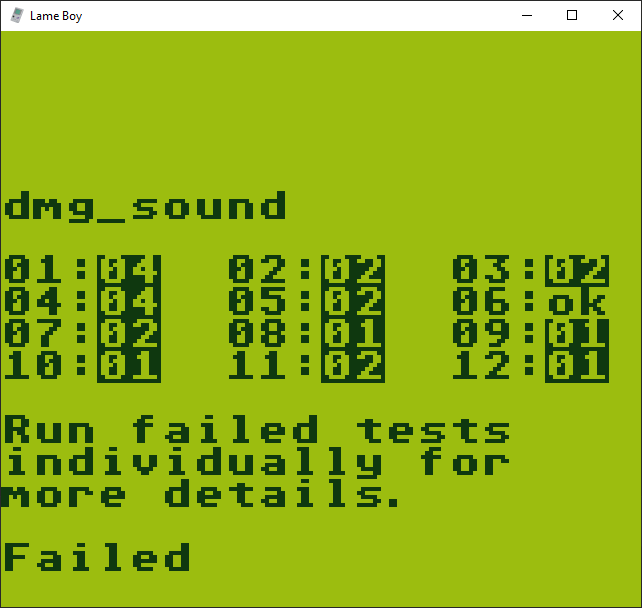
\includegraphics[width=\textwidth/2]{figures/APU/blargg_dmg_sound.PNG}
    \caption{Results of running the \texttt{dmg\_sound} test ROM from Blargg's test ROMs \cite{Blargg}.}
    \label{fig:blargg_dmg_sound}
\end{figure}
\newpage
\section{The Game Boy}
After having developed multiple microcontrollers, they were combined into a complete system as described in Section \ref{sec:resultsarchitecture}. This system is the public interface of the hardware units and could be considered the actual emulation of the Game Boy. In combining these microcontrollers an emulator is created which in its current state can run multiple games without issue and in many ways provide an authentic experience. The emulator does however display some irregularities and unwanted behaviour in certain games, both mechanical and visual.
\\\\
In code, this is represented by a separate ``GameBoy''-class which combines all of the developed microcontrollers. It is through this the emulation is run and through this, all information is funnelled to external libraries such as OpenGL, ImGui and OpenAL.

\begin{figure}[H]
    \centering
    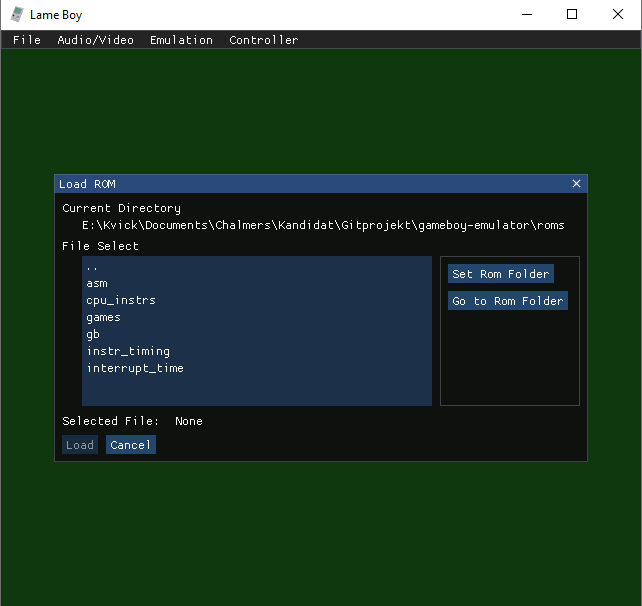
\includegraphics[width=0.7\textwidth]{figures/emulator.png}
    \caption{A screenshot of the emulator when loading ROMs.}
    \label{fig:emulator_picture}
\end{figure}